\documentclass[]{article}
\usepackage{lmodern}
\usepackage{amssymb,amsmath}
\usepackage{ifxetex,ifluatex}
\usepackage{fixltx2e} % provides \textsubscript
\ifnum 0\ifxetex 1\fi\ifluatex 1\fi=0 % if pdftex
  \usepackage[T1]{fontenc}
  \usepackage[utf8]{inputenc}
\else % if luatex or xelatex
  \ifxetex
    \usepackage{mathspec}
  \else
    \usepackage{fontspec}
  \fi
  \defaultfontfeatures{Ligatures=TeX,Scale=MatchLowercase}
\fi
% use upquote if available, for straight quotes in verbatim environments
\IfFileExists{upquote.sty}{\usepackage{upquote}}{}
% use microtype if available
\IfFileExists{microtype.sty}{%
\usepackage{microtype}
\UseMicrotypeSet[protrusion]{basicmath} % disable protrusion for tt fonts
}{}
\usepackage[margin=1in]{geometry}
\usepackage{hyperref}
\hypersetup{unicode=true,
            pdftitle={HW0\_Final.R},
            pdfauthor={James},
            pdfborder={0 0 0},
            breaklinks=true}
\urlstyle{same}  % don't use monospace font for urls
\usepackage{color}
\usepackage{fancyvrb}
\newcommand{\VerbBar}{|}
\newcommand{\VERB}{\Verb[commandchars=\\\{\}]}
\DefineVerbatimEnvironment{Highlighting}{Verbatim}{commandchars=\\\{\}}
% Add ',fontsize=\small' for more characters per line
\usepackage{framed}
\definecolor{shadecolor}{RGB}{248,248,248}
\newenvironment{Shaded}{\begin{snugshade}}{\end{snugshade}}
\newcommand{\KeywordTok}[1]{\textcolor[rgb]{0.13,0.29,0.53}{\textbf{#1}}}
\newcommand{\DataTypeTok}[1]{\textcolor[rgb]{0.13,0.29,0.53}{#1}}
\newcommand{\DecValTok}[1]{\textcolor[rgb]{0.00,0.00,0.81}{#1}}
\newcommand{\BaseNTok}[1]{\textcolor[rgb]{0.00,0.00,0.81}{#1}}
\newcommand{\FloatTok}[1]{\textcolor[rgb]{0.00,0.00,0.81}{#1}}
\newcommand{\ConstantTok}[1]{\textcolor[rgb]{0.00,0.00,0.00}{#1}}
\newcommand{\CharTok}[1]{\textcolor[rgb]{0.31,0.60,0.02}{#1}}
\newcommand{\SpecialCharTok}[1]{\textcolor[rgb]{0.00,0.00,0.00}{#1}}
\newcommand{\StringTok}[1]{\textcolor[rgb]{0.31,0.60,0.02}{#1}}
\newcommand{\VerbatimStringTok}[1]{\textcolor[rgb]{0.31,0.60,0.02}{#1}}
\newcommand{\SpecialStringTok}[1]{\textcolor[rgb]{0.31,0.60,0.02}{#1}}
\newcommand{\ImportTok}[1]{#1}
\newcommand{\CommentTok}[1]{\textcolor[rgb]{0.56,0.35,0.01}{\textit{#1}}}
\newcommand{\DocumentationTok}[1]{\textcolor[rgb]{0.56,0.35,0.01}{\textbf{\textit{#1}}}}
\newcommand{\AnnotationTok}[1]{\textcolor[rgb]{0.56,0.35,0.01}{\textbf{\textit{#1}}}}
\newcommand{\CommentVarTok}[1]{\textcolor[rgb]{0.56,0.35,0.01}{\textbf{\textit{#1}}}}
\newcommand{\OtherTok}[1]{\textcolor[rgb]{0.56,0.35,0.01}{#1}}
\newcommand{\FunctionTok}[1]{\textcolor[rgb]{0.00,0.00,0.00}{#1}}
\newcommand{\VariableTok}[1]{\textcolor[rgb]{0.00,0.00,0.00}{#1}}
\newcommand{\ControlFlowTok}[1]{\textcolor[rgb]{0.13,0.29,0.53}{\textbf{#1}}}
\newcommand{\OperatorTok}[1]{\textcolor[rgb]{0.81,0.36,0.00}{\textbf{#1}}}
\newcommand{\BuiltInTok}[1]{#1}
\newcommand{\ExtensionTok}[1]{#1}
\newcommand{\PreprocessorTok}[1]{\textcolor[rgb]{0.56,0.35,0.01}{\textit{#1}}}
\newcommand{\AttributeTok}[1]{\textcolor[rgb]{0.77,0.63,0.00}{#1}}
\newcommand{\RegionMarkerTok}[1]{#1}
\newcommand{\InformationTok}[1]{\textcolor[rgb]{0.56,0.35,0.01}{\textbf{\textit{#1}}}}
\newcommand{\WarningTok}[1]{\textcolor[rgb]{0.56,0.35,0.01}{\textbf{\textit{#1}}}}
\newcommand{\AlertTok}[1]{\textcolor[rgb]{0.94,0.16,0.16}{#1}}
\newcommand{\ErrorTok}[1]{\textcolor[rgb]{0.64,0.00,0.00}{\textbf{#1}}}
\newcommand{\NormalTok}[1]{#1}
\usepackage{graphicx,grffile}
\makeatletter
\def\maxwidth{\ifdim\Gin@nat@width>\linewidth\linewidth\else\Gin@nat@width\fi}
\def\maxheight{\ifdim\Gin@nat@height>\textheight\textheight\else\Gin@nat@height\fi}
\makeatother
% Scale images if necessary, so that they will not overflow the page
% margins by default, and it is still possible to overwrite the defaults
% using explicit options in \includegraphics[width, height, ...]{}
\setkeys{Gin}{width=\maxwidth,height=\maxheight,keepaspectratio}
\IfFileExists{parskip.sty}{%
\usepackage{parskip}
}{% else
\setlength{\parindent}{0pt}
\setlength{\parskip}{6pt plus 2pt minus 1pt}
}
\setlength{\emergencystretch}{3em}  % prevent overfull lines
\providecommand{\tightlist}{%
  \setlength{\itemsep}{0pt}\setlength{\parskip}{0pt}}
\setcounter{secnumdepth}{0}
% Redefines (sub)paragraphs to behave more like sections
\ifx\paragraph\undefined\else
\let\oldparagraph\paragraph
\renewcommand{\paragraph}[1]{\oldparagraph{#1}\mbox{}}
\fi
\ifx\subparagraph\undefined\else
\let\oldsubparagraph\subparagraph
\renewcommand{\subparagraph}[1]{\oldsubparagraph{#1}\mbox{}}
\fi

%%% Use protect on footnotes to avoid problems with footnotes in titles
\let\rmarkdownfootnote\footnote%
\def\footnote{\protect\rmarkdownfootnote}

%%% Change title format to be more compact
\usepackage{titling}

% Create subtitle command for use in maketitle
\providecommand{\subtitle}[1]{
  \posttitle{
    \begin{center}\large#1\end{center}
    }
}

\setlength{\droptitle}{-2em}

  \title{HW0\_Final.R}
    \pretitle{\vspace{\droptitle}\centering\huge}
  \posttitle{\par}
    \author{James}
    \preauthor{\centering\large\emph}
  \postauthor{\par}
      \predate{\centering\large\emph}
  \postdate{\par}
    \date{2019-04-13}


\begin{document}
\maketitle

\begin{Shaded}
\begin{Highlighting}[]
\KeywordTok{setwd}\NormalTok{(}\StringTok{"~/GitHub/MMSS_311_2"}\NormalTok{)}

\CommentTok{# Q1a) A vector with the numbers 1-5 in order }
\NormalTok{a <-}\StringTok{ }\KeywordTok{c}\NormalTok{(}\DecValTok{1}\NormalTok{,}\DecValTok{2}\NormalTok{,}\DecValTok{3}\NormalTok{,}\DecValTok{4}\NormalTok{,}\DecValTok{5}\NormalTok{)}

\CommentTok{# Q1b) A scalar named Mindy that takes the value 12}
\NormalTok{Mindy <-}\StringTok{ }\DecValTok{12}

\CommentTok{# Q1c) A 2×3 matrix with the numbers 1-6 in order by rows }
\NormalTok{b <-}\StringTok{ }\KeywordTok{c}\NormalTok{(}\DecValTok{1}\NormalTok{,}\DecValTok{2}\NormalTok{,}\DecValTok{3}\NormalTok{,}\DecValTok{4}\NormalTok{,}\DecValTok{5}\NormalTok{,}\DecValTok{6}\NormalTok{)}
\KeywordTok{matrix}\NormalTok{(b,}\DecValTok{2}\NormalTok{,}\DecValTok{3}\NormalTok{,}\OtherTok{TRUE}\NormalTok{)}
\end{Highlighting}
\end{Shaded}

\begin{verbatim}
##      [,1] [,2] [,3]
## [1,]    1    2    3
## [2,]    4    5    6
\end{verbatim}

\begin{Shaded}
\begin{Highlighting}[]
\CommentTok{# Q1d) A 2×3 matrix with the numbers 1-6 in order by columns }
\KeywordTok{matrix}\NormalTok{(b,}\DecValTok{2}\NormalTok{,}\DecValTok{3}\NormalTok{)}
\end{Highlighting}
\end{Shaded}

\begin{verbatim}
##      [,1] [,2] [,3]
## [1,]    1    3    5
## [2,]    2    4    6
\end{verbatim}

\begin{Shaded}
\begin{Highlighting}[]
\CommentTok{# Q1e) A 10×10 matrix of 1's }
\KeywordTok{matrix}\NormalTok{(}\DecValTok{1}\NormalTok{,}\DecValTok{10}\NormalTok{,}\DecValTok{10}\NormalTok{)}
\end{Highlighting}
\end{Shaded}

\begin{verbatim}
##       [,1] [,2] [,3] [,4] [,5] [,6] [,7] [,8] [,9] [,10]
##  [1,]    1    1    1    1    1    1    1    1    1     1
##  [2,]    1    1    1    1    1    1    1    1    1     1
##  [3,]    1    1    1    1    1    1    1    1    1     1
##  [4,]    1    1    1    1    1    1    1    1    1     1
##  [5,]    1    1    1    1    1    1    1    1    1     1
##  [6,]    1    1    1    1    1    1    1    1    1     1
##  [7,]    1    1    1    1    1    1    1    1    1     1
##  [8,]    1    1    1    1    1    1    1    1    1     1
##  [9,]    1    1    1    1    1    1    1    1    1     1
## [10,]    1    1    1    1    1    1    1    1    1     1
\end{verbatim}

\begin{Shaded}
\begin{Highlighting}[]
\CommentTok{# Q1f)  A vector consisting of the words THIS, IS, A, VECTOR (each word a separate element) }
\NormalTok{wordvec <-}\StringTok{ }\KeywordTok{c}\NormalTok{(}\StringTok{"THIS"}\NormalTok{, }\StringTok{"IS"}\NormalTok{, }\StringTok{"A"}\NormalTok{, }\StringTok{"VECTOR"}\NormalTok{)}

\CommentTok{# Q1g) A function that takes the sum of any three numbers }
\NormalTok{sum_of_three_numbers <-}\StringTok{ }\ControlFlowTok{function}\NormalTok{(x,y,z) \{}
\NormalTok{  x}\OperatorTok{+}\NormalTok{y}\OperatorTok{+}\NormalTok{z}
\NormalTok{\}}

\CommentTok{# Q1h) A function that takes one number as input, returns "Yes" if the number is less than or equal to 10 and "No" if the number is greater than 10}
\NormalTok{check <-}\StringTok{ }\ControlFlowTok{function}\NormalTok{(x) \{}
  \ControlFlowTok{if}\NormalTok{ (x}\OperatorTok{<=}\DecValTok{10}\NormalTok{) \{}
\NormalTok{    result <-}\StringTok{ "Yes"}
\NormalTok{  \}}
  \ControlFlowTok{else} \ControlFlowTok{if}\NormalTok{ (x}\OperatorTok{>}\DecValTok{10}\NormalTok{) \{}
\NormalTok{    result <-}\StringTok{ "No"}
\NormalTok{  \}}
  \KeywordTok{return}\NormalTok{(result)}
\NormalTok{\}}
\KeywordTok{check}\NormalTok{(}\DecValTok{9}\NormalTok{)}
\end{Highlighting}
\end{Shaded}

\begin{verbatim}
## [1] "Yes"
\end{verbatim}

\begin{Shaded}
\begin{Highlighting}[]
\CommentTok{# Q1i) Generate synthetic data by taking 1,000 draws from a normal distribution with a mean of 10 and a standard deviation of 1. Save these data to an object g.}
\NormalTok{g <-}\StringTok{ }\KeywordTok{rnorm}\NormalTok{(}\DecValTok{1000}\NormalTok{,}\DecValTok{10}\NormalTok{,}\DecValTok{1}\NormalTok{)}

\CommentTok{# Q1j) Create a separate object called y with 1,000 draws from a normal distribution with a mean of 5 and a standard deviation of 0.5. }
\NormalTok{y <-}\StringTok{ }\KeywordTok{rnorm}\NormalTok{(}\DecValTok{1000}\NormalTok{,}\DecValTok{5}\NormalTok{,}\FloatTok{0.5}\NormalTok{)}

\CommentTok{# Q1k)Generate a variable x with 1,000 values, where each value is a mean of 10 samples from g, with replacement. (Hint: use a for loop)}
\NormalTok{x =}\StringTok{ }\OtherTok{NULL}
\ControlFlowTok{for}\NormalTok{(i }\ControlFlowTok{in} \DecValTok{1}\OperatorTok{:}\DecValTok{1000}\NormalTok{) \{}
\NormalTok{  x [i] <-}\StringTok{ }\KeywordTok{mean}\NormalTok{(}\KeywordTok{sample}\NormalTok{(g, }\DecValTok{10}\NormalTok{, }\OtherTok{TRUE}\NormalTok{))}
\NormalTok{\}}

\CommentTok{# Q1)l Estimate a simple bivariate regression y on x and print your results. What do your results show?}
\CommentTok{# The results show that the OLS estimator of the coefficient of x is 0.02633, which is very small. This shows that there is only a weak positive correlation between y and x.}
\NormalTok{reg <-}\StringTok{ }\KeywordTok{lm}\NormalTok{(y }\OperatorTok{~}\StringTok{ }\NormalTok{x)}
\KeywordTok{print}\NormalTok{(reg)}
\end{Highlighting}
\end{Shaded}

\begin{verbatim}
## 
## Call:
## lm(formula = y ~ x)
## 
## Coefficients:
## (Intercept)            x  
##     4.41665      0.05605
\end{verbatim}

\begin{Shaded}
\begin{Highlighting}[]
\CommentTok{#Q2a Create an R script file that sets your working directory and loads the data. }
\KeywordTok{setwd}\NormalTok{(}\StringTok{"~/GitHub/MMSS_311_2"}\NormalTok{)}

\NormalTok{pums_chicago <-}\StringTok{ }\KeywordTok{read.csv}\NormalTok{(}\StringTok{"pums_chicago.csv"}\NormalTok{)}

\CommentTok{#2b How many variables are there in the dataset? }
\CommentTok{# There are 204 variables (from environment panel)}

\CommentTok{#2c What is the mean annual income, PINCP in this dataset?}
\NormalTok{PINCP_mean <-}\StringTok{ }\KeywordTok{mean}\NormalTok{(pums_chicago}\OperatorTok{$}\NormalTok{PINCP, }\DataTypeTok{na.rm =} \OtherTok{TRUE}\NormalTok{)}

\CommentTok{#2d Create a new variable in the PUMS dataframe called PINCP_LOG that is equal to the log of annual income. Were NaN values produced? Why?}
\CommentTok{#NaN values were produced because we cannot take log of 0, which is the value of some annual income observations.}
\NormalTok{pums_chicago}\OperatorTok{$}\NormalTok{PINCP_LOG <-}\StringTok{ }\KeywordTok{log}\NormalTok{(pums_chicago}\OperatorTok{$}\NormalTok{PINCP)}
\end{Highlighting}
\end{Shaded}

\begin{verbatim}
## Warning in log(pums_chicago$PINCP): NaNs produced
\end{verbatim}

\begin{Shaded}
\begin{Highlighting}[]
\CommentTok{#2e Create a new variable GRAD.DUMMY that takes the value “grad” if the respondent has any post-high school education, and “no grad” otherwise. Use the SCHL variable. }
\NormalTok{pums_chicago}\OperatorTok{$}\NormalTok{GRAD.DUMMY <-}\StringTok{ }\KeywordTok{ifelse}\NormalTok{(pums_chicago}\OperatorTok{$}\NormalTok{SCHL }\OperatorTok{>}\StringTok{ }\DecValTok{17}\NormalTok{, }\StringTok{"grad"}\NormalTok{, }\StringTok{"no grad"}\NormalTok{)}

\CommentTok{#2f Drop the variable SERIALNO from the dataset.}
\NormalTok{pums_chicago}\OperatorTok{$}\NormalTok{SERIALNO <-}\StringTok{ }\OtherTok{NULL}

\CommentTok{#2g Save your new dataset to a csv file in the working directory.}
\KeywordTok{write.csv}\NormalTok{(pums_chicago,}\StringTok{'editedPUMS_CHICAGO.csv'}\NormalTok{)}

\CommentTok{#2h Use the variable ESR, create 5 new dataframes: under 16, employed, unemployed, in the armed forces, and not in the labor force.}
\NormalTok{under16 <-}\StringTok{ }\NormalTok{pums_chicago[pums_chicago}\OperatorTok{$}\NormalTok{ESR }\OperatorTok{==}\StringTok{ "NA"}\NormalTok{, ]}
\NormalTok{employed <-}\StringTok{ }\NormalTok{pums_chicago[pums_chicago}\OperatorTok{$}\NormalTok{ESR }\OperatorTok\StringTok{ }\KeywordTok{c}\NormalTok{(}\StringTok{"1"}\NormalTok{, }\StringTok{"2"}\NormalTok{), ]}
\NormalTok{unemployed <-}\StringTok{ }\NormalTok{pums_chicago[pums_chicago}\OperatorTok{$}\NormalTok{ESR }\OperatorTok\StringTok{ "3"}\NormalTok{, ]}
\NormalTok{armedforces <-}\StringTok{ }\NormalTok{pums_chicago[pums_chicago}\OperatorTok{$}\NormalTok{ESR }\OperatorTok\StringTok{ }\KeywordTok{c}\NormalTok{(}\StringTok{"4"}\NormalTok{, }\StringTok{"5"}\NormalTok{), ]}
\NormalTok{notinlaborforce <-}\StringTok{ }\NormalTok{pums_chicago[pums_chicago}\OperatorTok{$}\NormalTok{ESR }\OperatorTok\StringTok{ "6"}\NormalTok{, ]}

\CommentTok{#2i Create a new dataframe that combines employed people and people in the armed forces. }
\NormalTok{employed_af <-}\StringTok{ }\NormalTok{pums_chicago[pums_chicago}\OperatorTok{$}\NormalTok{ESR }\OperatorTok\StringTok{ }\KeywordTok{c}\NormalTok{(}\StringTok{"1"}\NormalTok{, }\StringTok{"2"}\NormalTok{, }\StringTok{"4"}\NormalTok{, }\StringTok{"5"}\NormalTok{), ]}

\CommentTok{#2j In your new employed_af dataframe, keep only the variables AGEP, RAC1P, and PINCP_LOG}
\NormalTok{new_employed_af <-}\StringTok{ }\NormalTok{pums_chicago[}\KeywordTok{c}\NormalTok{(}\StringTok{"AGEP"}\NormalTok{, }\StringTok{"RAC1P"}\NormalTok{, }\StringTok{"PINCP_LOG"}\NormalTok{)]}

\CommentTok{#2ki Find the mean, median, and 80th percentile of travel time to work, JWMNP }
\KeywordTok{summary}\NormalTok{(pums_chicago}\OperatorTok{$}\NormalTok{JWMNP)}
\end{Highlighting}
\end{Shaded}

\begin{verbatim}
##    Min. 1st Qu.  Median    Mean 3rd Qu.    Max.    NA's 
##    1.00   20.00   30.00   34.84   45.00  149.00   27668
\end{verbatim}

\begin{Shaded}
\begin{Highlighting}[]
\KeywordTok{quantile}\NormalTok{(pums_chicago}\OperatorTok{$}\NormalTok{JWMNP, }\DataTypeTok{probs=}\FloatTok{0.8}\NormalTok{, }\DataTypeTok{na.rm=}\OtherTok{TRUE}\NormalTok{)}
\end{Highlighting}
\end{Shaded}

\begin{verbatim}
## 80% 
##  45
\end{verbatim}

\begin{Shaded}
\begin{Highlighting}[]
\CommentTok{#2kii Find the correlation between travel time to work JWMNP and annual wages WAGP }
\KeywordTok{cor}\NormalTok{(pums_chicago}\OperatorTok{$}\NormalTok{JWMNP, pums_chicago}\OperatorTok{$}\NormalTok{WAGP, }\DataTypeTok{use=}\StringTok{"complete.obs"}\NormalTok{)}
\end{Highlighting}
\end{Shaded}

\begin{verbatim}
## [1] -0.04205232
\end{verbatim}

\begin{Shaded}
\begin{Highlighting}[]
\CommentTok{#2kiii Make a scatterplot of age and log income.}
\CommentTok{#2kiv Export this graph to your working directory in pdf format.}
\KeywordTok{pdf}\NormalTok{(}\StringTok{"ageonLogincome.pdf"}\NormalTok{)}
\KeywordTok{plot}\NormalTok{(pums_chicago}\OperatorTok{$}\NormalTok{AGEP, pums_chicago}\OperatorTok{$}\NormalTok{PINCP_LOG, }\DataTypeTok{main=}\StringTok{"age on log income"}\NormalTok{)}
\KeywordTok{dev.off}\NormalTok{()}
\end{Highlighting}
\end{Shaded}

\begin{verbatim}
## pdf 
##   2
\end{verbatim}

\begin{Shaded}
\begin{Highlighting}[]
\CommentTok{#2kv Create a crosstab of employment status ESR by race RAC1P}
\KeywordTok{install.packages}\NormalTok{(}\StringTok{"gmodels"}\NormalTok{, }\DataTypeTok{repos =} \StringTok{"http://cran.us.r-project.org"}\NormalTok{)}
\end{Highlighting}
\end{Shaded}

\begin{verbatim}
## Installing package into 'C:/Users/James/Documents/R/win-library/3.5'
## (as 'lib' is unspecified)
\end{verbatim}

\begin{verbatim}
## package 'gmodels' successfully unpacked and MD5 sums checked
## 
## The downloaded binary packages are in
##  C:\Users\James\AppData\Local\Temp\Rtmp4c1HYH\downloaded_packages
\end{verbatim}

\begin{Shaded}
\begin{Highlighting}[]
\KeywordTok{library}\NormalTok{(}\StringTok{"gmodels"}\NormalTok{)}
\KeywordTok{CrossTable}\NormalTok{(pums_chicago}\OperatorTok{$}\NormalTok{ESR, pums_chicago}\OperatorTok{$}\NormalTok{RAC1P)}
\end{Highlighting}
\end{Shaded}

\begin{verbatim}
## 
##  
##    Cell Contents
## |-------------------------|
## |                       N |
## | Chi-square contribution |
## |           N / Row Total |
## |           N / Col Total |
## |         N / Table Total |
## |-------------------------|
## 
##  
## Total Observations in Table:  40348 
## 
##  
##                  | pums_chicago$RAC1P 
## pums_chicago$ESR |         1 |         2 |         3 |         4 |         5 |         6 |         7 |         8 |         9 | Row Total | 
## -----------------|-----------|-----------|-----------|-----------|-----------|-----------|-----------|-----------|-----------|-----------|
##                1 |     12870 |      5786 |        36 |         0 |        24 |      1746 |         7 |      2502 |       521 |     23492 | 
##                  |   195.313 |   406.565 |     0.689 |     1.164 |     0.414 |     9.555 |     0.591 |     4.491 |     3.239 |           | 
##                  |     0.548 |     0.246 |     0.002 |     0.000 |     0.001 |     0.074 |     0.000 |     0.107 |     0.022 |     0.582 | 
##                  |     0.659 |     0.447 |     0.507 |     0.000 |     0.511 |     0.627 |     0.778 |     0.607 |     0.630 |           | 
##                  |     0.319 |     0.143 |     0.001 |     0.000 |     0.001 |     0.043 |     0.000 |     0.062 |     0.013 |           | 
## -----------------|-----------|-----------|-----------|-----------|-----------|-----------|-----------|-----------|-----------|-----------|
##                2 |       258 |       147 |         0 |         0 |         0 |        31 |         0 |        66 |         8 |       510 | 
##                  |     0.487 |     1.687 |     0.897 |     0.025 |     0.594 |     0.502 |     0.114 |     3.730 |     0.576 |           | 
##                  |     0.506 |     0.288 |     0.000 |     0.000 |     0.000 |     0.061 |     0.000 |     0.129 |     0.016 |     0.013 | 
##                  |     0.013 |     0.011 |     0.000 |     0.000 |     0.000 |     0.011 |     0.000 |     0.016 |     0.010 |           | 
##                  |     0.006 |     0.004 |     0.000 |     0.000 |     0.000 |     0.001 |     0.000 |     0.002 |     0.000 |           | 
## -----------------|-----------|-----------|-----------|-----------|-----------|-----------|-----------|-----------|-----------|-----------|
##                3 |       794 |      1473 |         2 |         0 |         4 |       109 |         0 |       268 |        57 |      2707 | 
##                  |   204.029 |   420.880 |     1.603 |     0.134 |     0.227 |    32.435 |     0.604 |     0.252 |     0.041 |           | 
##                  |     0.293 |     0.544 |     0.001 |     0.000 |     0.001 |     0.040 |     0.000 |     0.099 |     0.021 |     0.067 | 
##                  |     0.041 |     0.114 |     0.028 |     0.000 |     0.085 |     0.039 |     0.000 |     0.065 |     0.069 |           | 
##                  |     0.020 |     0.037 |     0.000 |     0.000 |     0.000 |     0.003 |     0.000 |     0.007 |     0.001 |           | 
## -----------------|-----------|-----------|-----------|-----------|-----------|-----------|-----------|-----------|-----------|-----------|
##                4 |         4 |         5 |         0 |         0 |         0 |         0 |         1 |         0 |         1 |        11 | 
##                  |     0.331 |     0.613 |     0.019 |     0.001 |     0.013 |     0.759 |   405.558 |     1.123 |     2.661 |           | 
##                  |     0.364 |     0.455 |     0.000 |     0.000 |     0.000 |     0.000 |     0.091 |     0.000 |     0.091 |     0.000 | 
##                  |     0.000 |     0.000 |     0.000 |     0.000 |     0.000 |     0.000 |     0.111 |     0.000 |     0.001 |           | 
##                  |     0.000 |     0.000 |     0.000 |     0.000 |     0.000 |     0.000 |     0.000 |     0.000 |     0.000 |           | 
## -----------------|-----------|-----------|-----------|-----------|-----------|-----------|-----------|-----------|-----------|-----------|
##                6 |      5618 |      5533 |        33 |         2 |        19 |       899 |         1 |      1283 |       240 |     13628 | 
##                  |   146.443 |   308.317 |     3.392 |     2.597 |     0.615 |     1.846 |     1.369 |     8.421 |     5.537 |           | 
##                  |     0.412 |     0.406 |     0.002 |     0.000 |     0.001 |     0.066 |     0.000 |     0.094 |     0.018 |     0.338 | 
##                  |     0.287 |     0.427 |     0.465 |     1.000 |     0.404 |     0.323 |     0.111 |     0.311 |     0.290 |           | 
##                  |     0.139 |     0.137 |     0.001 |     0.000 |     0.000 |     0.022 |     0.000 |     0.032 |     0.006 |           | 
## -----------------|-----------|-----------|-----------|-----------|-----------|-----------|-----------|-----------|-----------|-----------|
##     Column Total |     19544 |     12944 |        71 |         2 |        47 |      2785 |         9 |      4119 |       827 |     40348 | 
##                  |     0.484 |     0.321 |     0.002 |     0.000 |     0.001 |     0.069 |     0.000 |     0.102 |     0.020 |           | 
## -----------------|-----------|-----------|-----------|-----------|-----------|-----------|-----------|-----------|-----------|-----------|
## 
## 
\end{verbatim}

\begin{Shaded}
\begin{Highlighting}[]
\CommentTok{#2kvi Estimate a linear regression of annual wages WAGP on hours worked per week WKHP }
\NormalTok{wagp_on_wkhp <-}\StringTok{ }\KeywordTok{lm}\NormalTok{(WAGP }\OperatorTok{~}\StringTok{ }\NormalTok{WKHP, pums_chicago)}

\CommentTok{#2kvii Plot the residuals from this regression against the fitted values. What does this show?}
\CommentTok{#This shows that residuals tend to decrease as the fitted values increase. Furthermore, we can observe that there are only a small number of large deviations for any given fitted value.}
\NormalTok{wagp_on_wkhp_res <-}\StringTok{ }\KeywordTok{resid}\NormalTok{(wagp_on_wkhp)}
\NormalTok{wagp_on_wkhp_fitted <-}\StringTok{ }\KeywordTok{fitted}\NormalTok{(wagp_on_wkhp)}
\KeywordTok{plot}\NormalTok{(wagp_on_wkhp_fitted, wagp_on_wkhp_res, }
     \DataTypeTok{ylab =} \StringTok{"Residuals"}\NormalTok{, }\DataTypeTok{xlab=}\StringTok{"Fitted"}\NormalTok{,}
     \DataTypeTok{main =} \StringTok{"Residuals on Fitted"}\NormalTok{)}

\CommentTok{#2li Estimate a linear regression of miles per gallon on weight }
\KeywordTok{data}\NormalTok{(mtcars)}
\NormalTok{car_lm <-}\StringTok{ }\KeywordTok{lm}\NormalTok{(mpg }\OperatorTok{~}\StringTok{ }\NormalTok{wt, mtcars)}

\CommentTok{#2lii Estimate this regression separately for manual versus automatic transition }
\NormalTok{autoData <-}\StringTok{ }\NormalTok{mtcars[mtcars}\OperatorTok{$}\NormalTok{am }\OperatorTok{==}\StringTok{ "0"}\NormalTok{,]}
\NormalTok{manualData <-}\StringTok{ }\NormalTok{mtcars[mtcars}\OperatorTok{$}\NormalTok{am }\OperatorTok{==}\StringTok{ "1"}\NormalTok{,]}
\NormalTok{autocar_lm <-}\StringTok{ }\KeywordTok{lm}\NormalTok{(mpg }\OperatorTok{~}\StringTok{ }\NormalTok{wt, mtcars)}
\NormalTok{manualcar_lm <-}\StringTok{ }\KeywordTok{lm}\NormalTok{(mpg }\OperatorTok{~}\StringTok{ }\NormalTok{wt, mtcars)}

\CommentTok{#2liii Estimate a regression of miles per gallon on the log of horsepower. }
\NormalTok{mtcars}\OperatorTok{$}\NormalTok{log.hp <-}\StringTok{ }\KeywordTok{log}\NormalTok{(mtcars}\OperatorTok{$}\NormalTok{hp)}
\NormalTok{mpg_on_lg.hp <-}\StringTok{ }\KeywordTok{lm}\NormalTok{(mpg }\OperatorTok{~}\StringTok{ }\NormalTok{log.hp, mtcars)}

\CommentTok{#2mi Make a scatterplot of weight against miles per gallon. }
\CommentTok{#2mii Color the points in your graph according to the transmission of the vehicle. }
\CommentTok{#2miii Change the shape of the points to correspond to the number of forward gears in the vehicle.}
\CommentTok{#2miv Change the x and y labels on the plot to make full words. }
\CommentTok{#2mv Change the background of the plot so that the panel background is not gray.}
\KeywordTok{install.packages}\NormalTok{(}\StringTok{"ggplot2"}\NormalTok{, }\DataTypeTok{repos =} \StringTok{"http://cran.us.r-project.org"}\NormalTok{)}
\end{Highlighting}
\end{Shaded}

\begin{verbatim}
## Installing package into 'C:/Users/James/Documents/R/win-library/3.5'
## (as 'lib' is unspecified)
\end{verbatim}

\begin{verbatim}
## package 'ggplot2' successfully unpacked and MD5 sums checked
## 
## The downloaded binary packages are in
##  C:\Users\James\AppData\Local\Temp\Rtmp4c1HYH\downloaded_packages
\end{verbatim}

\begin{Shaded}
\begin{Highlighting}[]
\KeywordTok{library}\NormalTok{(ggplot2)}
\end{Highlighting}
\end{Shaded}

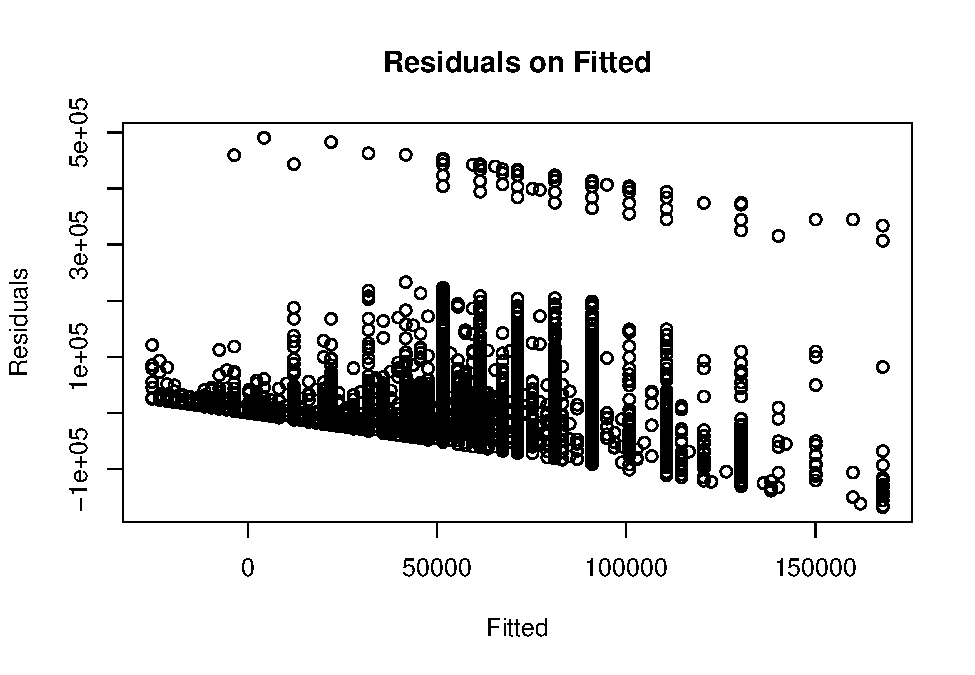
\includegraphics{HW0_Final_files/figure-latex/unnamed-chunk-1-1.pdf}

\begin{Shaded}
\begin{Highlighting}[]
\KeywordTok{ggplot}\NormalTok{(mtcars)}\OperatorTok{+}\StringTok{ }\KeywordTok{geom_point}\NormalTok{(}\DataTypeTok{mapping =} \KeywordTok{aes}\NormalTok{(}\DataTypeTok{x =}\NormalTok{ mpg, }\DataTypeTok{y =}\NormalTok{ wt, }
                                         \DataTypeTok{color =}\NormalTok{ mtcars}\OperatorTok{$}\NormalTok{am, }
                                         \DataTypeTok{shape =}\NormalTok{ mtcars}\OperatorTok{$}\NormalTok{gear)) }\OperatorTok{+}\StringTok{ }\KeywordTok{scale_shape_identity}\NormalTok{() }\OperatorTok{+}\StringTok{ }
\StringTok{  }\KeywordTok{labs}\NormalTok{(}\DataTypeTok{title =} \StringTok{"Weight on Miles per Gallon"}\NormalTok{, }\DataTypeTok{x =} \StringTok{"Miles per Gallon"}\NormalTok{, }\DataTypeTok{y =} \StringTok{"Weight"}\NormalTok{) }\OperatorTok{+}
\StringTok{  }\KeywordTok{theme}\NormalTok{(}\DataTypeTok{panel.background =} \KeywordTok{element_rect}\NormalTok{(}\DataTypeTok{fill =} \StringTok{"lightyellow"}\NormalTok{))}
\end{Highlighting}
\end{Shaded}

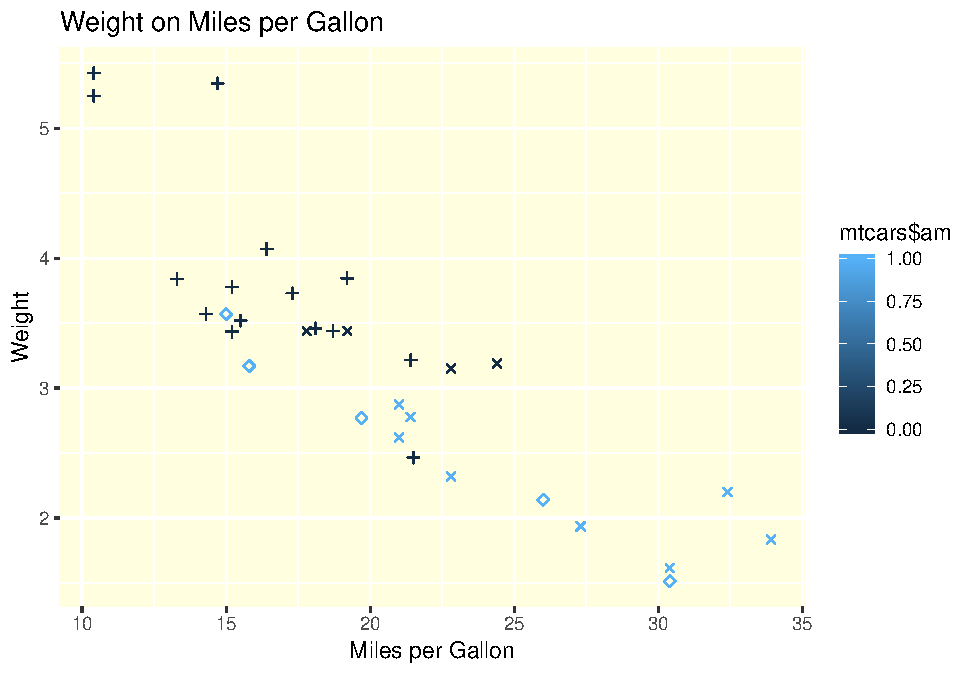
\includegraphics{HW0_Final_files/figure-latex/unnamed-chunk-1-2.pdf}


\end{document}
